% Oito minutos de apresentação e no máximo 10 slides

\documentclass{beamer}
\usepackage[brazil]{babel}
\usepackage[utf8]{inputenc}
\usepackage{xcolor}
\usepackage{verbatim}
\usepackage{tikz}
\usetikzlibrary {positioning}
\usetikzlibrary{arrows}

\tikzset{edge/.style = {->,> = latex'}}

    \graphicspath{
    {.} % document root dir
    {./img/}
}

\usetheme{Madrid}
\usecolortheme{beaver}

\title[Problema do Carteiro Chinês e Variantes]{O Problema do Carteiro Chinês e Variantes}
\author[Gabriel F. Oliveira]{Gabriel Fernandes de Oliveira\newline Prof. Carlos Eduardo Ferreira}
\institute[IME - USP]{Instituto de Matemática e Estatística}

\logo{
\includegraphics[height=1.5cm]{ime.png}}

\begin{document}

\setbeamertemplate{caption}{\raggedright\insertcaption\par}

\begin{frame}
    \titlepage
\end{frame}
    
%\begin{frame}{Sumário}
    %\tableofcontents
%\end{frame}

\begin{comment}
\section{Objetivos}

\begin{frame}{Objetivos}

    \begin{columns}
        \column{0.6\textwidth} 

        \begin{itemize}
            \item Estudar o problema do carteiro chinês
            \item Documentar resultados
            \item Implementar e disponibilizar soluções 
        \end{itemize}

        \column{0.4\textwidth}
            \center
            \begin{figure}
                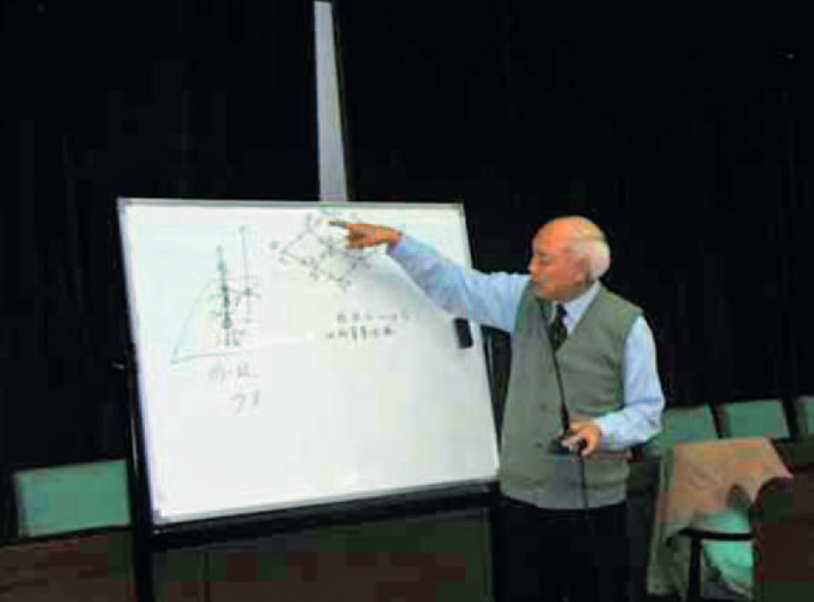
\includegraphics[width=.7\textwidth]{meigu.png}
                \caption{\small Mei-Ko Kwan}
            \end{figure}
            \begin{figure}
                 
\includegraphics[width=.5\textwidth]{github.png}
                 \caption{\small \href{https://github.com/gafeol/chinese-postman}{gafeol/chinese-postman}}
            \end{figure}
    \end{columns}

\end{frame}
\end{comment}

\section{Definição}

\begin{frame}{O problema do carteiro chinês}
    \begin{alertblock}{Definição}
        Encontrar uma rota fechada, de menor custo, que percorre toda aresta de um grafo ao menos uma vez.
    \end{alertblock}


    \begin{figure}
        \centering
        \begin{tikzpicture}[auto,node distance=3cm, every loop/.style={},thick,main node/.style={circle,draw,font=\sffamily\Large}]
            \node[main node] (1) []{1};
            \node[main node] (2) [below of=1] {2};
            \node[main node] (3) [right of=2] {3};
            \node[main node] (4) [right of=1] {4};

            \path[every node/.style={font=\sffamily\small}]
                (1) edge node [right] {2} (2)
                (1) edge node [] {1} (3)
                (1) edge node [above] {1} (4)
                (3) edge node [above] {2} (2)
                (4) edge node [left] {3} (3)
                ;
        \end{tikzpicture}
    \end{figure}

\end{frame}


\begin{frame}{O problema do carteiro chinês}
    \begin{alertblock}{Definição}
        Encontrar uma rota fechada, de menor custo, que percorre toda aresta de um grafo ao menos uma vez.
    \end{alertblock}

    \begin{figure}
        \centering
        \begin{tikzpicture}[auto,node distance=3cm, every loop/.style={},thick,main node/.style={circle,draw,font=\sffamily\Large}]
            \node[main node] (1) []{1};
            \node[main node] (2) [below of=1] {2};
            \node[main node] (3) [right of=2] {3};
            \node[main node] (4) [right of=1] {4};

            \path[->] (1) edge[blue] node[above] {1} (4);
            %\path[->] (4) edge node[left] {3} (3);
            %\path[->] (3) edge[] node[above] {2} (2);

            %\path[->] (3) edge[bend right=15] node[above] {2} (2);
            %\path[->] (3) edge[bend left=15, red] node[above] {2} (2);

            %\path[->] (2) edge[] node[right] {2} (1);

            %\path[->] (2) edge[bend right=15] node[right] {2} (1);
            %\path[->] (2) edge[bend left=15, red] node[right] {2} (1);

            %\path[->] (1) edge node[above] {1} (3);
            \path[every node/.style={font=\sffamily\small}]
                (1) edge node [right] {2} (2)
                (1) edge node [] {1} (3)
                %(1) edge node [above] {1} (4)
                (3) edge node [above] {2} (2)
                (4) edge node [left] {3} (3)
                ;
        \end{tikzpicture}
        %\caption{Custo de rota: 13}
    \end{figure}
\end{frame}
\begin{frame}{O problema do carteiro chinês}
    \begin{alertblock}{Definição}
        Encontrar uma rota fechada, de menor custo, que percorre toda aresta de um grafo ao menos uma vez.
    \end{alertblock}

    \begin{figure}
        \centering
        \begin{tikzpicture}[auto,node distance=3cm, every loop/.style={},thick,main node/.style={circle,draw,font=\sffamily\Large}]
            \node[main node] (1) []{1};
            \node[main node] (2) [below of=1] {2};
            \node[main node] (3) [right of=2] {3};
            \node[main node] (4) [right of=1] {4};

            \path[->] (1) edge[blue] node[above] {1} (4);
            \path[->] (4) edge[blue] node[left] {3} (3);
            %\path[->] (3) edge[] node[above] {2} (2);

            %\path[->] (3) edge[bend right=15] node[above] {2} (2);
            %\path[->] (3) edge[bend left=15, red] node[above] {2} (2);

            %\path[->] (2) edge[] node[right] {2} (1);

            %\path[->] (2) edge[bend right=15] node[right] {2} (1);
            %\path[->] (2) edge[bend left=15, red] node[right] {2} (1);

            %\path[->] (1) edge node[above] {1} (3);
            \path[every node/.style={font=\sffamily\small}]
                (1) edge node [right] {2} (2)
                (1) edge node [] {1} (3)
                %(1) edge node [above] {1} (4)
                (3) edge node [above] {2} (2)
                %(4) edge node [left] {3} (3)
                ;
        \end{tikzpicture}
        %\caption{Custo de rota: 13}
    \end{figure}

\end{frame}

\begin{frame}{O problema do carteiro chinês}
    \begin{alertblock}{Definição}
        Encontrar uma rota fechada, de menor custo, que percorre toda aresta de um grafo ao menos uma vez.
    \end{alertblock}

    \begin{figure}
        \centering
        \begin{tikzpicture}[auto,node distance=3cm, every loop/.style={},thick,main node/.style={circle,draw,font=\sffamily\Large}]
            \node[main node] (1) []{1};
            \node[main node] (2) [below of=1] {2};
            \node[main node] (3) [right of=2] {3};
            \node[main node] (4) [right of=1] {4};

            \path[->] (1) edge[blue] node[above] {1} (4);
            \path[->] (4) edge[blue] node[left] {3} (3);
            \path[->] (3) edge[blue] node[above] {2} (2);

            %\path[->] (3) edge[bend right=15] node[above] {2} (2);
            %\path[->] (3) edge[bend left=15, red] node[above] {2} (2);

            %\path[->] (2) edge[] node[right] {2} (1);

            %\path[->] (2) edge[bend right=15] node[right] {2} (1);
            %\path[->] (2) edge[bend left=15, red] node[right] {2} (1);

            %\path[->] (1) edge node[above] {1} (3);
            \path[every node/.style={font=\sffamily\small}]
                (1) edge node [right] {2} (2)
                (1) edge node [] {1} (3)
                %(1) edge node [above] {1} (4)
                %(3) edge node [above] {2} (2)
                %(4) edge node [left] {3} (3)
                ;
        \end{tikzpicture}
        %\caption{Custo de rota: 13}
    \end{figure}

\end{frame}
\begin{frame}{O problema do carteiro chinês}
    \begin{alertblock}{Definição}
        Encontrar uma rota fechada, de menor custo, que percorre toda aresta de um grafo ao menos uma vez.
    \end{alertblock}

    \begin{figure}
        \centering
        \begin{tikzpicture}[auto,node distance=3cm, every loop/.style={},thick,main node/.style={circle,draw,font=\sffamily\Large}]
            \node[main node] (1) []{1};
            \node[main node] (2) [below of=1] {2};
            \node[main node] (3) [right of=2] {3};
            \node[main node] (4) [right of=1] {4};

            \path[->] (1) edge[blue] node[above] {1} (4);
            \path[->] (4) edge[blue] node[left] {3} (3);
            \path[->] (3) edge[blue] node[above] {2} (2);
            \path[->] (2) edge[blue] node[right] {2} (1);

            %\path[->] (3) edge[bend right=15] node[above] {2} (2);
            %\path[->] (3) edge[bend left=15, red] node[above] {2} (2);


            %\path[->] (2) edge[bend right=15] node[right] {2} (1);
            %\path[->] (2) edge[bend left=15, red] node[right] {2} (1);

            %\path[->] (1) edge node[above] {1} (3);
            \path[every node/.style={font=\sffamily\small}]
                (1) edge node [] {1} (3)
                ;
        \end{tikzpicture}
        %\caption{Custo de rota: 13}
    \end{figure}

\end{frame}
\begin{frame}{O problema do carteiro chinês}
    \begin{alertblock}{Definição}
        Encontrar uma rota fechada, de menor custo, que percorre toda aresta de um grafo ao menos uma vez.
    \end{alertblock}

    \begin{figure}
        \centering
        \begin{tikzpicture}[auto,node distance=3cm, every loop/.style={},thick,main node/.style={circle,draw,font=\sffamily\Large}]
            \node[main node] (1) []{1};
            \node[main node] (2) [below of=1] {2};
            \node[main node] (3) [right of=2] {3};
            \node[main node] (4) [right of=1] {4};

            \path[->] (1) edge[blue] node[above] {1} (4);
            \path[->] (4) edge[blue] node[left] {3} (3);
            \path[->] (3) edge[blue] node[above] {2} (2);
            \path[->] (2) edge[blue] node[right] {2} (1);
            \path[->] (1) edge[blue] node[above] {1} (3);

            %\path[->] (3) edge[bend right=15] node[above] {2} (2);
            %\path[->] (3) edge[bend left=15, red] node[above] {2} (2);


            %\path[->] (2) edge[bend right=15] node[right] {2} (1);
            %\path[->] (2) edge[bend left=15, red] node[right] {2} (1);

        \end{tikzpicture}
        %\caption{Custo de rota: 13}
    \end{figure}
\end{frame}
\begin{frame}{O problema do carteiro chinês}
    \begin{alertblock}{Definição}
        Encontrar uma rota fechada, de menor custo, que percorre toda aresta de um grafo ao menos uma vez.
    \end{alertblock}

    \begin{figure}
        \centering
        \begin{tikzpicture}[auto,node distance=3cm, every loop/.style={},thick,main node/.style={circle,draw,font=\sffamily\Large}]
            \node[main node] (1) []{1};
            \node[main node] (2) [below of=1] {2};
            \node[main node] (3) [right of=2] {3};
            \node[main node] (4) [right of=1] {4};

            \path[->] (1) edge[blue] node[above] {1} (4);
            \path[->] (4) edge[blue] node[left] {3} (3);
            \path[->] (2) edge[blue] node[right] {2} (1);
            \path[->] (1) edge[blue] node[above] {1} (3);

            \path[->] (3) edge[blue, bend right=15] node[above] {2} (2);
            \path[->] (3) edge[red, bend left=15, red] node[above] {2} (2);


            %\path[->] (2) edge[bend right=15] node[right] {2} (1);
            %\path[->] (2) edge[bend left=15, red] node[right] {2} (1);

        \end{tikzpicture}
        %\caption{Custo de rota: 13}
    \end{figure}

\end{frame}
\begin{frame}{O problema do carteiro chinês}
    \begin{alertblock}{Definição}
        Encontrar uma rota fechada, de menor custo, que percorre toda aresta de um grafo ao menos uma vez.
    \end{alertblock}

    \begin{figure}
        \centering
        \begin{tikzpicture}[auto,node distance=3cm, every loop/.style={},thick,main node/.style={circle,draw,font=\sffamily\Large}]
            \node[main node] (1) []{1};
            \node[main node] (2) [below of=1] {2};
            \node[main node] (3) [right of=2] {3};
            \node[main node] (4) [right of=1] {4};

            \path[->] (1) edge[blue] node[above] {1} (4);
            \path[->] (4) edge[blue] node[left] {3} (3);
            \path[->] (1) edge[blue] node[above] {1} (3);

            \path[->] (3) edge[blue, bend right=15] node[above] {2} (2);
            \path[->] (3) edge[red, bend left=15, red] node[above] {2} (2);

            \path[->] (2) edge[blue, bend right=15] node[right] {2} (1);
            \path[->] (2) edge[red, bend left=15, red] node[right] {2} (1);

        \end{tikzpicture}
        \caption{Custo de rota: 13}
    \end{figure}
\end{frame}
\begin{frame}{O problema do carteiro chinês}
    \begin{alertblock}{Definição}
        Encontrar uma rota fechada, de menor custo, que percorre toda aresta de um grafo ao menos uma vez.
    \end{alertblock}

    \centering

    \scalebox{0.85}{
        \begin{columns}
            \column{0.5\textwidth}

            \begin{figure}
                \centering
                \begin{tikzpicture}[auto,node distance=3cm, every loop/.style={},thick,main node/.style={circle,draw,font=\sffamily\Large}]
                    \node[main node] (1) []{1};
                    \node[main node] (2) [below of=1] {2};
                    \node[main node] (3) [right of=2] {3};
                    \node[main node] (4) [right of=1] {4};

                    \path[->] (1) edge node[above] {1} (4);
                    \path[->] (4) edge node[left] {3} (3);
                    \path[->] (3) edge[bend right=15] node[above] {2} (2);
                    \path[->] (3) edge[bend left=15, red] node[above] {2} (2);
                    \path[->] (2) edge[bend right=15] node[right] {2} (1);
                    \path[->] (2) edge[bend left=15, red] node[right] {2} (1);
                    \path[->] (1) edge node[above] {1} (3);
                \end{tikzpicture}
                \caption{Custo de rota: 13}
            \end{figure}

            \column{0.5\textwidth}

            \begin{figure}
                \centering
                \begin{tikzpicture}[auto,node distance=3cm, every loop/.style={},thick,main node/.style={circle,draw,font=\sffamily\Large}]
                    \node[main node] (1) []{1};
                    \node[main node] (2) [below of=1] {2};
                    \node[main node] (3) [right of=2] {3};
                    \node[main node] (4) [right of=1] {4};

                    \path[->] (1) edge node[above] {1} (4);
                    \path[->] (4) edge node[left] {3} (3);
                    \path[->] (3) edge node[above] {2} (2);
                    \path[->] (2) edge node[right] {2} (1);
                    \path[->] (1) edge[bend right=15] node[above] {1} (3);
                    \path[->] (3) edge[bend right=15, red] node[above] {1} (1);
                \end{tikzpicture}
                \caption{Custo de rota: 10}
            \end{figure}
        \end{columns}
    }

    \begin{center}
        Objetivo: minimizar o custo das \textcolor{red}{arestas repetidas} na rota.
    \end{center}
\end{frame}

\section{Solução}

\begin{frame}{Solução do problema do carteiro chinês}
    \begin{itemize}
        \item Em \textbf{grafos eulerianos}, as soluções ótimas são circuitos eulerianos.
        \item No caso geral, constrói-se um supergrafo euleriano, cujo circuito euleriano resolve o problema.
    \end{itemize}

    \vspace{10px}

    \begin{alertblock}{Definição: Grafo euleriano}

        \begin{columns}
            \column{0.6\textwidth}
            Grafo que possui um circuito que percorre todas suas arestas sem repetições. 

            \column{0.3\textwidth}
            \begin{figure}
                \centering
                \begin{tikzpicture}[auto,node distance=1cm, every loop/.style={},thick,main node/.style={circle,draw,font=\sffamily\footnotesize}]
                    \node[main node] (1) [] {};
                    \node[main node] (2) [below left of=1] {};
                    \node[main node] (3) [below right of=1] {};

                    \path[->] (1) edge node {} (2);
                    \path[->] (2) edge node {} (3);
                    \path[->] (3) edge node {} (1);
                \end{tikzpicture}
            \end{figure}
            \vspace{3px}
        \end{columns}
    \end{alertblock}

\end{frame}

\begin{frame}{Solução do problema do carteiro chinês}{Caso geral em grafos não eulerianos}

    \begin{columns}[T]
        \column{.45\textwidth}
        \begin{figure}
            \centering
            \begin{tikzpicture}[auto,node distance=2.5cm, every loop/.style={},thick,main node/.style={circle,draw,font=\tiny}]
                \node[main node, red] (1) [] {};
                \node[main node, red] (2) [below of=1] {};
                \node[main node] (3) [right of=2] {};
                \node[main node, blue] (4) [right of=1] {};

                \path[->] (1) edge[bend right=10] node {} (4);
                \path[->] (4) edge[bend right=10] node {} (1);
                \path[->] (1) edge[] node {} (2);
                \path[->] (2) edge[] node {} (3);
                \path[->] (3) edge[] node {} (4);
                \path[->] (2) edge[] node {} (4);
            \end{tikzpicture}
        \end{figure}

        Grau de entrada $\neq$ Grau de saída

        \column{.45\textwidth}
        \begin{figure}
            \centering
            \begin{tikzpicture}[auto,node distance=2.5cm, every loop/.style={},thick,main node/.style={circle,draw,font=\sffamily\footnotesize}]
                \node[main node, red] (1) [] {};
                \node[main node] (2) [below of=1] {};
                \node[main node, red] (3) [right of=2] {};
                \node[main node] (4) [right of=1] {};

                \path[every node/.style={font=\sffamily\small}]
                    (1) edge node [right] {} (2)
                    (1) edge node [] {} (3)
                    (1) edge node [above] {} (4)
                    (3) edge node [above] {} (2)
                    (4) edge node [left] {} (3)
                    ;
            \end{tikzpicture}
        \end{figure}

        \centering
        Vértices com \textcolor{red}{grau ímpar}
    \end{columns}

\end{frame}

\begin{frame}{Solução do problema do carteiro chinês}{Caso geral em grafos não eulerianos}
        

    \begin{columns}[T]
        \column{.45\textwidth}
        \begin{figure}
            \centering
            \begin{tikzpicture}[auto,node distance=2.5cm, every loop/.style={},thick,main node/.style={circle,draw,font=\tiny}]
                \node[main node, red] (1) [] {-1};
                \node[main node, red] (2) [below of=1] {-1};
                \node[main node] (3) [right of=2] {};
                \node[main node, blue] (4) [right of=1] {+2};

                \path[->] (1) edge[bend right=10] node {} (4);
                \path[->] (4) edge[bend right=10] node {} (1);
                \path[->] (1) edge[] node {} (2);
                \path[->] (2) edge[] node {} (3);
                \path[->] (3) edge[] node {} (4);
                \path[->] (2) edge[] node {} (4);
            \end{tikzpicture}
        \end{figure}

        Problema de transporte.

        Definem-se \textcolor{blue}{oferta} e \textcolor{red}{demanda}, de acordo com o grau dos vértices.

        \column{.45\textwidth}

        \begin{figure}
            \centering
            \begin{tikzpicture}[auto,node distance=2.5cm, every loop/.style={},thick,main node/.style={circle,draw,font=\sffamily\footnotesize}]
                \node[main node, red] (1) [] {};
                \node[main node] (2) [below of=1] {};
                \node[main node, red] (3) [right of=2] {};
                \node[main node] (4) [right of=1] {};

                \path[every node/.style={font=\sffamily\small}]
                    (1) edge node [right] {} (2)
                    (1) edge node [] {} (3)
                    (1) edge node [above] {} (4)
                    (3) edge node [above] {} (2)
                    (4) edge node [left] {} (3)
                    ;
            \end{tikzpicture}
        \end{figure}

        Emparelhamento perfeito entre vértices de \textcolor{red}{grau ímpar}.
    \end{columns}

\end{frame}

\begin{frame}{Solução do problema do carteiro chinês}{Caso geral em grafos não eulerianos}
        
    As arestas duplicadas tornam os grafos eulerianos

    \begin{columns}[T]
        \column{.45\textwidth}
        \begin{figure}
            \centering
            \begin{tikzpicture}[auto,node distance=2.5cm, every loop/.style={},thick,main node/.style={circle,draw,font=\tiny}]
                \node[main node] (1) [] {};
                \node[main node] (2) [below of=1] {};
                \node[main node] (3) [right of=2] {};
                \node[main node] (4) [right of=1] {};

                \path[->] (1) edge[bend right=10] node {} (4);
                \path[->] (4) edge[bend right=10] node {} (1);
                \path[->] (4) edge[bend right=30, red] node {} (1);
                \path[->] (4) edge[bend right=50, red] node {} (1);
                \path[->] (1) edge[bend left=10] node {} (2);
                \path[->] (1) edge[bend right=10, red] node {} (2);
                \path[->] (2) edge[] node {} (3);
                \path[->] (3) edge[] node {} (4);
                \path[->] (2) edge[] node {} (4);
            \end{tikzpicture}
        \end{figure}

        \column{.45\textwidth}

        \vspace{17px}

        \begin{figure}
            \centering
            \begin{tikzpicture}[auto,node distance=2.5cm, every loop/.style={},thick,main node/.style={circle,draw,font=\sffamily\footnotesize}]
                \node[main node] (1) [] {};
                \node[main node] (2) [below of=1] {};
                \node[main node] (3) [right of=2] {};
                \node[main node] (4) [right of=1] {};

                \path[every node/.style={font=\sffamily\small}]
                    (1) edge node [right] {} (2)
                    (1) edge[bend left=10] node [] {} (3)
                    (1) edge[bend right=10, red] node [] {} (3)
                    (1) edge node [above] {} (4)
                    (3) edge node [above] {} (2)
                    (4) edge node [left] {} (3)
                    ;
            \end{tikzpicture}
        \end{figure}

    \end{columns}

    \vspace{10px}

    As arestas artificiais são as arestas repetidas na rota que soluciona o problema do carteiro chinês.

\end{frame}

\section{Variantes}

\begin{frame}{Variantes}
    Todas variações estudadas são NP-completas.

    \begin{columns}

        \column{0.7\textwidth}
        \begin{itemize}
            \item \textbf{Grafos mistos}
                \begin{itemize}
                    \item 2-aproximação - Frederickson (1979).
                    \item Aplica emparelhamento perfeito e o problema de transporte.
                \end{itemize}

        \end{itemize}

        \column{0.3\textwidth}

        \begin{figure}
            \centering
            \begin{tikzpicture}[auto,node distance=1.5cm, every loop/.style={},thick,main node/.style={circle,draw,font=\sffamily\footnotesize}]
                \node[main node] (1) [] {};
                \node[main node] (2) [below of=1] {};
                \node[main node] (3) [right of=2] {};
                \node[main node] (4) [right of=1] {};

                \path[->] (1) edge node[] {} (4);
                \path[->] (4) edge node[] {} (2);
                \path[every node/.style={font=\sffamily\small}]
                    (1) edge node [right] {} (2)
                    (1) edge node [] {} (3)
                    (3) edge node [above] {} (2)
                    (4) edge node [left] {} (3)
                    ;
            \end{tikzpicture}
        \end{figure}
        
    \end{columns}
\end{frame}

\begin{frame}{Variantes}

    \begin{columns}

        \column{0.7\textwidth}
        \begin{itemize}

            \item \textbf{Rural}

                Nem todas arestas/arcos precisam ser percorridos.
                \begin{itemize}
                    \item $\frac{3}{2}$-aproximação - Christofides (1976/1986).  
                    \item Emparelhamento a partir uma árvore/arborescência geradora mínima.
                \end{itemize}

        \end{itemize}

        \column{0.3\textwidth}

        \begin{figure}
            \centering
            \begin{tikzpicture}[auto,node distance=1.5cm, every loop/.style={},thick,main node/.style={circle,draw,font=\sffamily\footnotesize}]
                \node[main node] (1) [] {};
                \node[main node] (2) [below of=1] {};
                \node[main node] (3) [right of=2] {};
                \node[main node] (4) [right of=1] {};
                \node[main node] (5) at (2.25, -0.75) [] {};

                \path[every node/.style={font=\sffamily\small}]
                    (1) edge[dotted] node [] {} (4)
                    (1) edge node [right] {} (2)
                    (1) edge[dotted] node [] {} (3)
                    (3) edge[dotted] node [above] {} (2)
                    (4) edge node [left] {} (3)
                    (5) edge node [] {} (3)
                    (5) edge[dotted] node [] {} (4)
                    ;
            \end{tikzpicture}
        \end{figure}
    \end{columns}
\end{frame}

\begin{frame}{Variantes}
    \begin{itemize}
        \item \textbf{Com ruas íngremes (ou com vento)}

            Custos diferentes para cada orientação de uma aresta.

            \begin{itemize}
                \item Caso especial: custo de todo circuito é o mesmo independente da direção em que são percorridos.
                \item Solução polinomial - Mei-Ko Kwan (1983)
                \item Reduz para o problema do carteiro chinês original.
            \end{itemize}
    \end{itemize}
        \center
        \begin{tikzpicture}[auto,node distance=1.5cm, every loop/.style={},thick,main node/.style={circle,draw,font=\sffamily\footnotesize}]
            \node[main node] (1) [] {u};
            \node[main node] (2) [right of=1] {v};
            \path[every node/.style={font=\sffamily\small}]
                (1) edge node {\textcolor{blue}{2}/\textcolor{red}{3}} (2);
        \end{tikzpicture}

        \begin{columns}
            \column{0.2\textwidth}
            \begin{figure}
                \centering
                \begin{tikzpicture}[auto,node distance=1.5cm, every loop/.style={},thick,main node/.style={circle,draw,font=\sffamily\footnotesize}]
                    \node[main node] (1) [] {u};
                    \node[main node] (2) [right of=1] {v};
                    \path[->] (1) edge[blue] node[above] {2} (2);
                \end{tikzpicture}
            \end{figure}

            \column{0.2\textwidth}

            \begin{figure}
                \centering
                \begin{tikzpicture}[auto,node distance=1.5cm, every loop/.style={},thick,main node/.style={circle,draw,font=\sffamily\footnotesize}]
                    \node[main node] (1) [] {u};
                    \node[main node] (2) [right of=1] {v};
                    \path[->] (2) edge[red] node[above] {3} (1);
                \end{tikzpicture}
            \end{figure}
        \end{columns}

        \vspace{5px}

        \begin{tikzpicture}[auto,node distance=1.5cm, every loop/.style={},thick,main node/.style={circle,draw,font=\sffamily\footnotesize}]
            \node[main node] (1) [] {u};
            \node[main node] (2) [right of=1] {v};
            \path[every node/.style={font=\sffamily\small}]
                (1) edge node {2.5} (2);
        \end{tikzpicture}

\end{frame}
\section{Resultados}

\begin{frame}{Resultados}
    \begin{columns}
        \column{0.7\textwidth}
        \begin{itemize}
            \item \href{https://www.linux.ime.usp.br/~gafeol/mac0499/chinese-postman/tex/main.pdf}{Monografia disponibilizada}
            \item Implementações em C++17
            \item Documentação de código
            \item 132 testes, 99.6\% cobertura
            \item Testes automatizados
        \end{itemize} 

        \vspace{5px}

        \begin{center}
            \href{https://github.com/gafeol/chinese-postman}{\texttt{github.com/gafeol/chinese-postman}}
            \href{https://www.linux.ime.usp.br/~gafeol/mac0499/}{\texttt{linux.ime.usp.br/$\sim$gafeol/mac0499}}
            
        \end{center}

        \column{0.25\textwidth}

        \center
        \begin{figure}
            
\includegraphics[width=0.5\textwidth]{cpp.png}
        \end{figure}
        \begin{figure}
            
\includegraphics[width=0.5\textwidth]{travis.png}
        \end{figure}
        
    \end{columns}

\end{frame}


\end{document}
